\section{Attack Mechanics}
Given that:
\begin{enumerate}
    \item IOMMU hardware is correctly implemented 
    \item IOMMU is correctly initialized on time
\end{enumerate}
One might assume that the systems are safe from DMA attacks. We contend that this is not the case. The \textit{least-privilege principle} requires that an entity such as a software module or a physical device must always have only the minimum necessary access to operate normally. In this chapter, we describe the risks caused by software when this principle is violated.
\subsection{MMO}\label{sec:mmo}
In this section we introduce the notion of MMO (Motive,Means,Opportunity) in the context of DMA attacks. Using the idea we can better understand the vulnerabilities of the OS and the viability of possible prevention methods. In order to gain control over a server the malicious device needs three things:
\begin{enumerate}
    \item Motive: The device has DMA access, to what should be a restricted area. The malicious device is now motivated to exploit this situation. 
    \item Means: The device has a valid \kva of a \mabaf. The device wields the \kva as a weapon.
    \item Opportunity: The device can overwrite a callback pointer in a deterministic way. The device has a target in its cross-hairs.
\end{enumerate}
For example, a NIC has write access to a page of an RX packet. Due to sub page vulnerability a random structure with a callback pointer is accessible at a random offset. While this may seem, that the device has a valid attack vector it is actually missing two key ingredients. The device has no \textit{Means}. While the device can write a \mabaf on to the page; the device must figure out the \kva\footnote{The device is using an IOVA to access memory, to the best of our knowledge there is no way to correlate an IOVA to a \kva on a Linux machine}. The device also doesn't have an \textit{Opportunity}. Without  read access or any other additional information, the NIC cant know what structures are exposed and at what offsets. While corrupting random kernel memory may cause a kernel panic \cite{MMT16}, but its not the goal that we are after.

\begin{figure}[t]
    \centering
    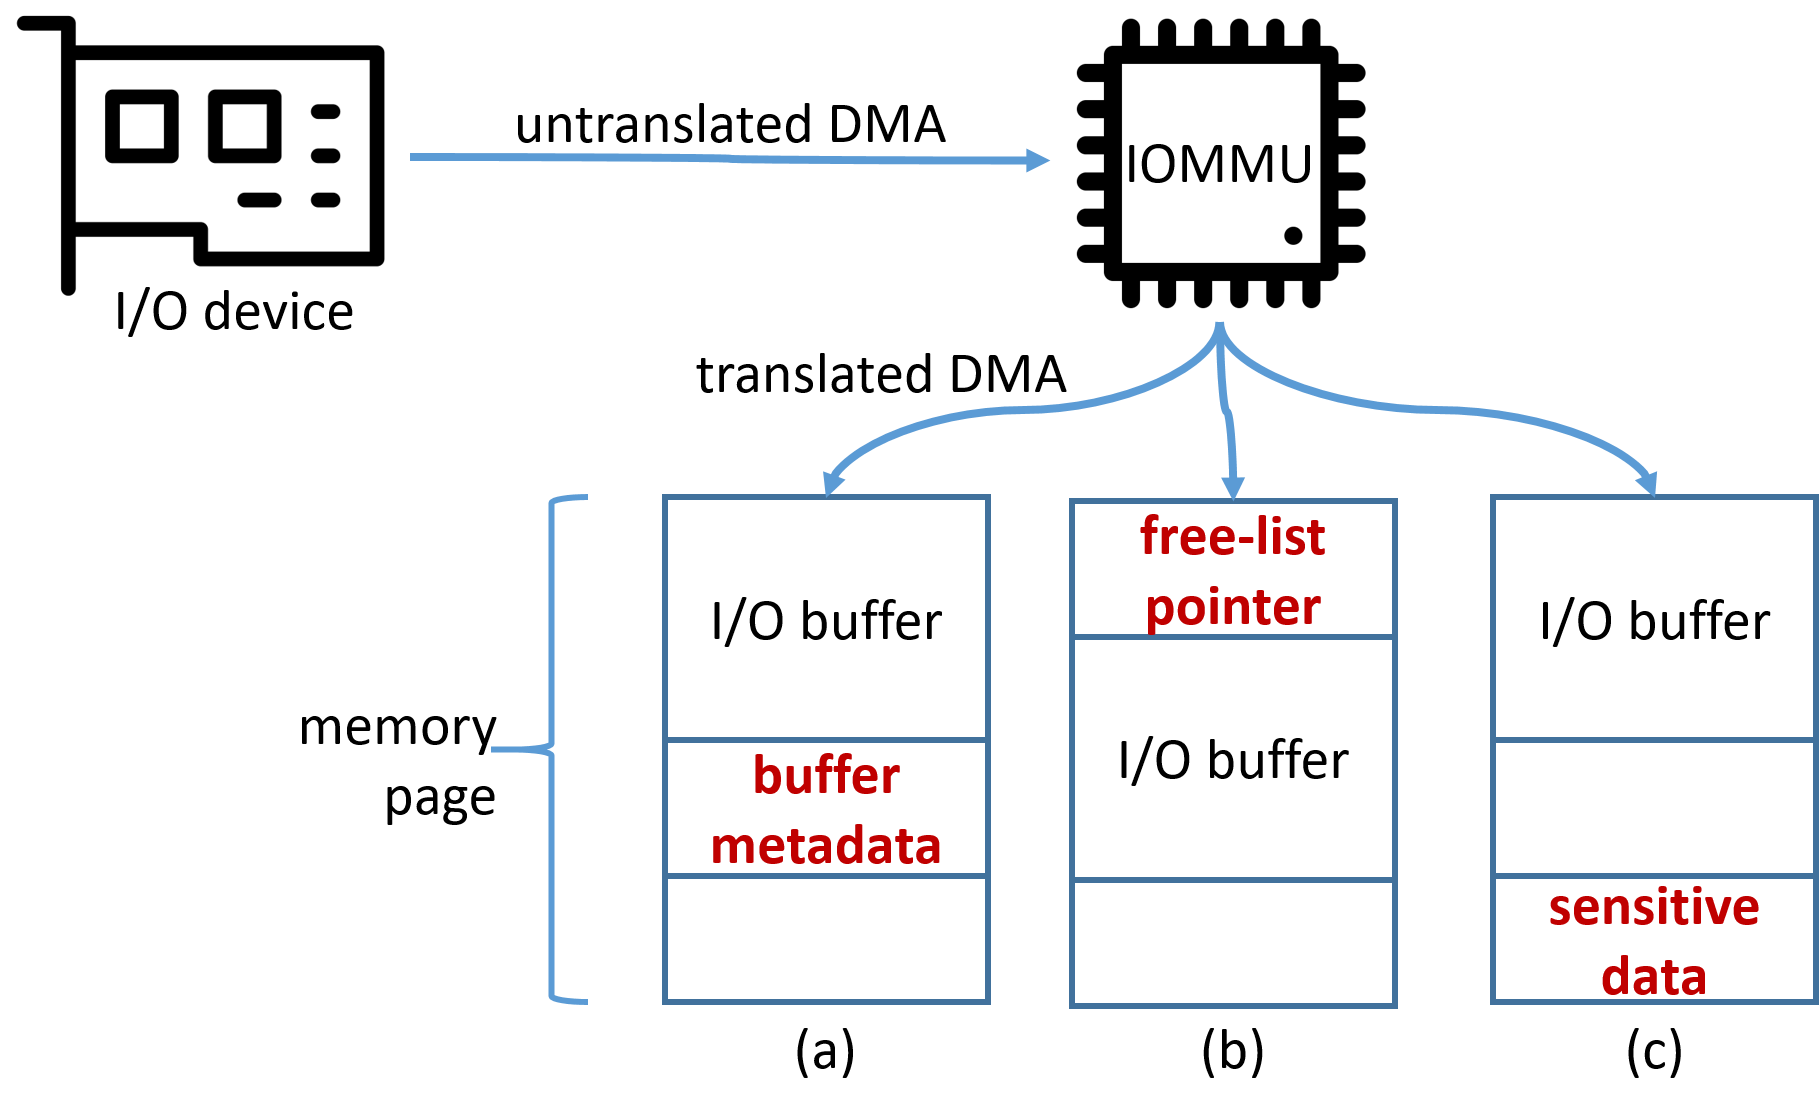
\includegraphics[width=1\columnwidth]{figs/colocation.png}
    \caption{Sub-page granularity DMA vulnerabilities when the I/O buffer resides in
a page that also holds other data: (a) I/O buffer metadata, (b) memory allocator’s
metadata such as free-list pointers and (c) randomly colocated sensitive buffers.}
    \label{fig:colocation}
\end{figure}
\subsection{Sub-Page}\label{sec:subpage}
Currently, OSs allocate I/O buffer memory using the same mechanisms they use for any memory allocation. These mechanisms, however, are oblivious to the role of the allocated memory. Consequently, I/O buffers may reside in the same page with other and potentially sensitive data. Since IOMMU protection is limited to page granularity, I/O devices that are allowed to access an I/O buffer gain access to this data as well. This behavior might compromise the system security. We classified the different types of potentially co-located data into three categories (as illustrated in Figure ~\ref{fig:colocation}: In case (a), the I/O buffer is part of a bigger data structure that also contains metadata used by the device driver. In the extreme case, this metadata might include function pointers, which enable relatively simple and robust attacks. Other fields in such data structures might be dangerous as well. In case (b), the memory allocator saves metadata, such as free-lists, with the I/O buffers, in the same page \cite{Cor07}. Manipulating these data structures may compromise the system completely \cite{ak09}. Finally, in (c), the I/O buffer and another dynamically allocated memory may reside in the same page. This common situation can easily cause data leakage, but may also be used for more sophisticated attacks. 
%We used randomly colocated pointers to break kASLR, as we discuss in Chapter 5. Why do OSs ignore the disparity between I/O buffer allocation alignment and protection granularity? One possible explanation is the benefits of dense memory allocations: lower internal memory fragmentation, which results in higher memory utilization, and lower translation lookaside buffer (TLB) pressure, which reduces the number of TLB misses. We suspect, however, that the main reason for the disparity is actually more prosaic. As IOMMUs were introduced to commodity servers relatively recently, OS developers have been reluctant to overhaul existing device drivers and change the way they allocate and manage their memory. Instead, IOMMU mapping operations were abstracted from device drivers, and implemented on top of existing DMA APIs [MHJ, The]. As a result, the memory allocation of I/O buffers has not been modified and adapted to take into consideration the IOMMU protection granularity.
\subsection{Deferred Invalidation vulnerability} 
\begin{figure*}[t]
    \centering
    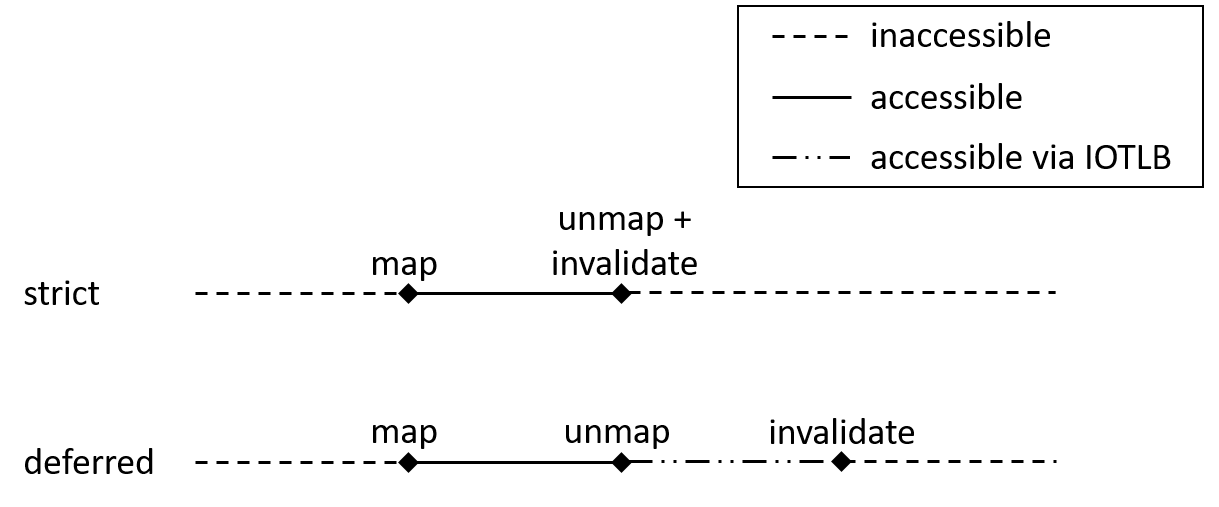
\includegraphics[width=1.3\columnwidth]{figs/deferred.png}
    \caption{Strict vs. deferred IOTLB invalidations. In deferred mode, there is a period
where the data is accessible but the mapping no longer exists.}
    \label{fig:deferred}
\end{figure*}
To translate addresses efficiently, the IOMMU caches translations in an input/output translation lookaside buffer (IOTLB). Like MMUs, IOMMUs do not maintain consistency between the IOTLB and the IOMMU page tables, which reside in memory; instead, the OS is required to restore consistency by explicitly invalidating the IOTLB. Therefore, to ensure that the IOTLB never holds stale entries, the OS must invalidate the IOTLB immediately after it removes memory mappings. Yet this scheme, called the “strict” mode in Linux, can degrade performance, as IOTLB invalidations can induce very high overhead \cite{MMT16,MSMT18,Peleg15}. In I/O intensive workloads, the number of required IOTLB invalidations can be extremely high, as IOMMU entries are unmapped following each I/O operation. Moreover, the overhead of each IOTLB invalidation can be as high as 2000 cycles \cite{ABYTS11}, considerably more than TLB invalidation, which takes roughly 100 cycles \cite{Han14}. To reduce this overhead, Linux defers TLB invalidations by default, and instead performs periodic global TLB invalidations. This “deferred” mode induces smaller performance overheads relative to the alternative “strict” mode. Nevertheless, as depicted in Figure \ref{fig:deferred}, deferring IOTLB invalidations may not prevent I/O devices from accessing unmapped pages, as the IOMMU may perform translations using stale IOTLB entries until the actual invalidation. This behavior introduces a security hazard, as the OS can reuse pages for other purposes after they are unmapped, regardless of the actual time of IOTLB invalidation. In the time window between the unmap operation and the actual invalidation, the OS may place sensitive data in the unmapped page-frame which the device may then read or modify. This time frame may be as high as 10 milliseconds when I/O traffic is low \cite{MSMT18}. In fact, this is a common scenario, as OSs prefer to reuse “hot” page-frames, recently freed, as they are likely to be already cached in the CPU caches\cite{hotcold}
. Therefore, it is possible in certain cases to predict how unmapped memory would be reused and which data it would expose.  
%As we demonstrate in Section 4.3, this behavior enables us to build robust assaults powerful enough to gain full control over a victim system.
\subsection{Threat Model}
Our attacks are built on the following assumptions:
\begin{enumerate}
    \item The actual attack is performed by a DMA-capable malicious device.
    \item There is software that violates the least-privilege principle with respect to the I/O device. The inherent vulnerabilities in the common use of the IOMMU make this a realistic assumption (§\ref{sec:sbp2_attack}). 
 \end{enumerate}
 The attacks discussed in this work are not executed by modifying the victim’s OS or drivers. We also assume that any hardware aside from the specific malicious device is working as expected, especially the DMA controller and the IOMMU itself. We also do not consider ports intended for debugging (e.g., jtag).
\subsection{Consequences}
The greatest potential consequence of our attacks is privilege escalation, which allows attackers to execute arbitrary code with kernel privileges. In all our experiments, we successfully executed code in the context of the kernel. Another, potential consequence is full system memory; these are harder to thwart and even harder to detect.  
Lastly, a consequence of a simple attack is denial of service \cite{MMT16}; where we crush the OS. Ideally, malformed devices should not be able to crash the entire system. The IOMMU is expected to properly isolate the devices from the OS to ensure this does not happen. Bad isolation, such as colocation of different types of data in the same page, may lead to system instability. To reach the above results, the attacker must have write permissions to some memory region. When an attacker has only read permissions, the consequences may still be interesting as they may lead to data leakage\cite{thunder}. The kernel often keeps sensitive data such as encryption keys and passwords as plain-text in memory. Attackers may use incorrect read permissions to leak this sensitive information.